\thispagestyle{empty}
\BgThispage
\begin{center}
    \LARGE
    \textbf{Software Requirements Specification \\
    (Спецификация требований к продукту)} \\
    \normalsize
\end{center}

\begin{enumerate}
    \item \textbf{Introduction (Введение)}
\begin{enumerate}[label=1.\arabic*]
        \item Purpose \\
        Цель документа заключается в определении требований к реализуемому продукту, используемых технологий,
        методологий и накладываемых ограничений. Описание процесса разработки и эксплуатирования с возможными издержками.
        \item Scope (Область применения) \\
        Данный документ относится к проекту ``Эхо Петербурга'' - сетевому партнеру радиостанции ``Эхо Москвы''. Документ
        создан для использования разработчиками, дизайнерами, тестировщиками, заказчиками
        \item Definitions, Acronyms and Abbreviations (Определения и аббревиатуры) \\
        JavaScript - язык программирования, который используют разработчики для создания интерактивных веб-страниц. \\
        PHP - язык программирования общего назначения, интенсивно применяемый для разработки веб-приложений. \\
        TCP/IP - сетевая модель передачи данных, представленных в цифровом виде. \\
        API - (интерфейс прикладного программирования) - это набор определенных правил, которые позволяют различным приложениям взаимодействовать друг с другом. \\
        Внедрение SQL-кода - один из распространённых способов взлома сайтов и программ, работающих с базами данных, основанный на внедрении в запрос произвольного SQL-кода. \\
        Внедрение HTML-кода - способ взлома сайтов и программ, путём ручного редактирования кода элемента страницы. \\
        Cookie - небольшой фрагмент данных, отправленный веб-сервером и хранимый на компьютере пользователя.\\
        Backup - процесс создания копии данных на носителе (жёстком диске, дискете и т. д.), предназначенном для восстановления данных в оригинальном или новом месте их расположения в случае их повреждения или разрушения. \\
        Front-end - презентационная часть информационной или программной системы, её пользовательский интерфейс и связанные с ним компоненты (та часть, что видит пользователь). \\
        Interface - совокупность средств, методов и правил взаимодействия (управления, контроля и т. д.) между элементами системы. \\
        User Interface - интерфейс, обеспечивающий передачу информации между пользователем-человеком и программно-аппаратными компонентами котьютерной системы. \\
        User friendly interface - это программный интерфейс, в котором пользователь может легко понимать приложение и эффективно перемещаться по нему. \\
        DoS (Denial of Service ``отказ в обслуживании'') - хакерская атака на вычислительную систему с целью довести её до отказа. \\
        DDoS - Если атака выполняется одновременно с большого числа компьютеров, говорят о DDoS-атаке. Такая атака проводится в том случае, если требуется вызвать отказ в обслуживании хорошо защищённой крупной компании или правительственной организации.
        \item References (Ссылки) \\
        \url{https://echomsk.spb.ru}  - главный домен сервиса
        \item Overview (Обзор документа) \\
        Общее описание - Данный раздел содержит описание факторов, влияющих на требования к продукту, сами требования
        отписываются в следующем разделе. \\
        Спецификация требований- Данный раздел содержит описание всех требований к разрабатываемой системе. Данное
        описание будет использоваться как разработчиками при разработке системы, так и тестировщиками в процессе проверки ее функционала
    \end{enumerate}
    \item \textbf{Overall Description (Общее описание)}
    \begin{enumerate}[label=2.\arabic*]
        \item Product functions (Функциональность продукта) \\
        ``Эхо Петербурга'' - это сетевое издание, которое предоставляет точную, оперативную и полную информации в
        виде новостей или статистики 24 часа в сутки 7 дней в неделю.
        \item User characteristics (Описание пользователей) \\
        Посетители сайта ( читатели ) - это люди, которые переходят на сайт ``Эхо Петербурга'' в браузере, ищут и
        читают новости и статистику по Covid-19, делятся новостями в соц.сетях и переходят на сайты-источники новостей.
        \item Assumptions and dependencies (Влияющие факторы и зависимости) \\
        User friendly interface (выполнение Usability требований) \\
        Быстрая подгрузка контента (выполнение Usability и Performance требований)\\
        Наличие иллюстраций к новостям \\
        Популярность новостного портала \\
        Круглосуточная работа сайта (выполнение Reliability требований)
        \item Сonstraints (Ограничения) \\
        На портале отсутствует индектификация пользователей, а значит нет персональных подборок. \\
        Для того, чтобы поделиться новостью или перейти в источник, необходимо перейти на расширенную версию новости.
    \end{enumerate}
    \BgThispage
    \item \textbf{Specific Requirements (Спецификация требований)}
    \begin{enumerate}[label=3.\arabic*]
        \item Functionality (Функциональные требования)
        \begin{enumerate}[label=3.1.\arabic*]
            \item Система должна предоставлять информацию в виде новостей, собирать статистику по самым популярным новостям.
            \item Система должна предоставлять пользователю возможность выполнять поиск новостей по тегам.
            \item Система должна предоставлять пользователю возможность выполнять поиск по совпадению слов в новостях.
            \item Система должна предоставлять пользователю возможность выполнять фильтрацию новостей по категориям.
            \item Система должна предоставлять пользователю превью новости, и возможность перейти к расширенному взаимодействию с новостью.
            \item Система должна предоставлять пользователю возможность поделиться новостью в соц. сетях.
            \item Система должна предоставлять пользователю возможность перейти к источнику новости.
            \item Система должна предоставлять пользователю возможность просматривать ежедневно обновляемую статистику по заболеваемости COVID-19
            \item Система должна предоставлять пользователю возможность оставить обратную связь.
        \end{enumerate}
\BgThispage
        \item Usability (Требования к удобству использования)
        \begin{enumerate}[label=3.2.\arabic*]
            \item Система должна обладать интуитивно понятным интерфейсом (неопытный (стаж использования ПК 1-3 года) пользователь должен свободно ориентироваться во всех разделах и возможностях сайта).
            \item В системе должны быть выделены и вынесены отдельно тематики новостей.
            \item В системе должен быть выделен топ новостей.
            \item Страница должна в среднем прогружаться за 2-5 секунд при интернет-соединении 100 Мбит/сек.
            \item В системе должна отсутствовать реклама.
        \end{enumerate}
        \newpage
        \item Reliability (Требования к надежности)
        \begin{enumerate}[label=3.3.\arabic*]
            \item Cистема должна работать без перебоев 24/7, не считая часы профилактики. Профилактические работы каждый вторник с 12 до 14, направленные на поддержание работоспособности, внедрение обновлений, исправление багов.
            \item В случае непредвиденной критической ошибки система должна восстанавливаться и загружаться из бэкапа не более чем за 3 минуты, запускаться не более чем 10 минут.
            \item Система должна обладать защитой от DOS и DDOS атак.
            \item Система должна обладать защитой от sql-внедрений.
            \item Система должна обладать защитой от html-внедрений.
%            \item Система должна стабильно функционировать при резком наплыве пользователей (х2 от предполагаемой нагрузки в 5 тыс. одновременных пользователей).
        \end{enumerate}
        \item Performance (Требования к производительности)
        \begin{enumerate}[label=3.4.\arabic*]
            \item Система должна отвечать на запросы пользователя не дольше 5 секунд.
            \item Система должна иметь среднее время ответа 3 секунды.
            \item Система должна стабильно обрабатывать 200 транзакций в секунду. \\
            \tiny \textit{(2 млн жителей ленобласти - 300 тыс. детей, из них 10\% заходит на сайт, /24/60/60 секунд и *50 средних запросов в день *2 для надёжности)}
            \normalsize
            \item Система должна стабильно одновременно обслуживать 5000 пользователей.
            \tiny \textit{(один запрос в среднем раз в 20 секунд, +1000 для надёжности)}
            \normalsize
        \end{enumerate}
        \item Design Constraints (Ограничения разработки) \\
        Система должна иметь адаптивную вёрстку. \\
        Во front-end части системы должен использоваться JavaScript. \\
        В серверной части системы должен использоваться PHP для обработки запросов пользователей.
        \item Interfaces (Интерфейсы)
        \BgThispage
        \begin{enumerate}[label=3.6.\arabic*]
            \item User Interfaces (Пользовательские интерфейсы): \\
            На главной странице сайта гость видит шапку, содержащую логотип, поиск и кнопку с выпадающим меню.
            Выпадающее меню появляется слева и содержит навигацию по сайту. По центру главной страницы
            располагается главная новость дня, занимающая 50\% пространства по вертикали. Сбоку от главной
            новости располагается топ новостей. Под главной новостью расположены ссылки на отфильтрованные
            новости по тегам.В нижней части страницы расположены превью всех новостей за данный день, отсортированные
            по времени добавления. Превью новостей содержат дату и время добавления, название новости, изображение и начало новости. \\
            \newpage
            Страница со статистикой Covid-19 содержит таблицу с числом заболевших, выздоровевших и умерших от covid-19 за текущие сутки. \\
            На странице ``Контакты'' расположена форма для обратной связи, содержащая поля для записи почты, имени и сообщения, а также кнопку ``отправить''. Под формой расположена информация о редакции и о команде проекта. \\
            На странице ``Политика конфиденциальности'' находится положение о COOKIE и обработке персональных данных. \\
            На странице ``Соглашение'' расположены Правила использования материалов сайта echomsk.spb.ru .
            \item Hardware Interfaces (Аппаратные интерфейсы): \\
            64gb ram. \\
            2 xeon 64 ядер 3.0 GHz. \\
            2 ТБ на все необходимое ПО, бэкап сервисы, память под сам бэкап etc.
            \item Software Interfaces (Программные интерфейсы): \\
            API Facebook/Twitter/VK/Pinterest/reddit content publishing
            \item Communications Interfaces (Сетевые интерфейсы): \\
%            HTTPS REST API
        \end{enumerate}
        \item Licensing Requirements (Требования к лицензированию) \\
        \BgThispage
        Лицензия сетевого издания реестра зарегистрированных СМИ (ФС77 - 38973) (( истек , иностранный агент)) \\
        Система распространяется под проприетарной лицензией. Раскрытие и использование исходных кодов программ и прочих компонентов системы разрешается исключительно с письменного согласия владельцев продукта.
    \end{enumerate}
\end{enumerate}
\vspace{1cm}
\begin{center}
    \large
    \textbf{Атрибуты функциональных \\ требований\\}
    \small
    \begin{tabular}{|l|l|l|l|l|}
        \hline
        N\textsuperscript{\underline{o}} & Требование                              & Приоритетность & Чел./ч & Риски*  \\
        \hline
        1                                & Предоставление новостей                 & Критическая    & 8      & Низкие  \\
        \hline
        2                                & Cбор статистики по просмотрам           & Средняя        & 8      & Низкие  \\
        \hline
        3                                & Поиск по тегам                          & Низкая         & 6      & Низкие  \\
        \hline
        4                                & Поиск по совпадающим словам             & Низкая         & 4      & Низкие  \\
        \hline
        5                                & Фильтрация по категориям                & Низкая         & 4      & Низкие  \\
        \hline
        6                                & Переход от превью к расширенной новости & Высокая        & 4      & Средние \\
        \hline
        7                                & Sharing в соц. сети                     & Средняя        & 6      & Высокие \\
        \hline
        8                                & Переход к источнику новости             & Критическая    & 2      & Высокие \\
        \hline
        9                                & Статистика по COVID-19                  & Высокая        & 6      & Средние \\
        \hline
        10                               & Возможность обратной связи              & Средняя        & 4      & Низкие  \\
        \hline
    \end{tabular}
\end{center}
\newpage
\BgThispage
\large
\begin{center}
    \textbf{Атрибуты нефункциональных требований\\}
\end{center}
\begin{center}
    \small
    \begin{tabular}{|l|l|l|l|l|}
        \hline
        N\textsuperscript{\underline{o}} & Требование                      & Приоритетность & Чел./ч & Риски*  \\
        \hline
        1                                & Выделить топ новостей           & Высокая        & 4      & Высокие \\
        \hline
        2                                & Загрузка страницы за 2-5 сек    & Критическая    & 8      & Высокие \\
        \hline
        3                                & Отсутсвие рекламы               & Высокая        & 0      & Низкие  \\
        \hline
        4                                & Стабильная работа системы       & Критическая    & 16     & Высокие \\
        \hline
        5                                & Защита от хакеров               & Высокая        & 30     & Средние \\
        \hline
        6                                & Обработка ~200 транзакций/сек   & Высокая        & 16     & Средние \\
        \hline
        7                                & Оптимизация памяти пользователя & Средняя        & 12     & Высокие \\
        \hline
        8                                & Адаптивная вёрстка              & Критическая    & 6      & Низкие  \\
        \hline
    \end{tabular}\\
    \vspace{1cm}
    \large
    \textbf{Прецеденты\\}
    \small
    \begin{tabular}{|l|l|}
        \hline
        Имя                   & Искать новость                                \\
        \hline
        ID                    & 1                                             \\
        \hline
        Описание              & Пользователь сайта осуществляет поиск новости \\
        \hline
        Актеры                & Пользователь                                  \\
        \hline
        Основной поток        & Пользователь выбирает инструмент для поиска,  \\
        & ищет новость и выбирает интересующую          \\
        \hline
        Постусловия           & -                                             \\
        \hline
        Альтернативные потоки & -                                             \\
        \hline
    \end{tabular}\\
    \vspace{0.5cm}
    \begin{tabular}{|l|l|}
        \hline
        Имя                   & Искать новость по тегам                        \\
        \hline
        ID                    & 1.1                                            \\
        \hline
        Описание              & Пользователь сайта осуществляет поиск новости, \\
        & выбирая нужный тег                             \\
        \hline
        Актеры                & Пользователь                                   \\
        \hline
        Основной поток        & Пользователь выбирает нужный тег,              \\
        & нажимает на него, скроллит страницу с          \\
        & новостями и выбирает интересующую              \\
        \hline
        Постусловия           & -                                              \\
        \hline
        Альтернативные потоки & -                                              \\
        \hline
    \end{tabular}\\
    \vspace{0.5cm}
    \begin{tabular}{|l|l|}
        \hline
        Имя                   & Искать новость в поисковой строке              \\
        \hline
        ID                    & 1.2                                            \\
        \hline
        Описание              & Пользователь сайта осуществляет поиск          \\
        & новости в поисковой строке                     \\
        \hline
        Актеры                & Пользователь                                   \\
        \hline
        Основной поток        & Пользователь нажимает на значок поиска, вводит \\
        & название новости или ключевые слова и выбирает \\
        & интересующую новость из результата поиска      \\
        \hline
        Постусловия           & -                                              \\
        \hline
        Альтернативные потоки & -                                              \\
        \hline
    \end{tabular}
\end{center}
\newpage
\BgThispage
1000-7?
\begin{center}
    \small
    \begin{tabular}{|l|l|}
        \hline
        Имя                   & Искать новость по темам                             \\
        \hline
        ID                    & 1.3                                                 \\
        \hline
        Описание              & Пользователь сайта осуществляет поиск новости,      \\
        & выбирая нужную тему                                 \\
        \hline
        Актеры                & Пользователь                                        \\
        \hline
        Основной поток        & Пользователь выбирает нужную тему в шапке страницы, \\
        & нажимает на него, скроллит страницу                 \\
        & с новостями и выбирает интересующую                 \\
        \hline
        Постусловия           & -                                                   \\
        \hline
        Альтернативные потоки & -                                                   \\
        \hline
    \end{tabular}\\
    \vspace{0.5cm}
    \begin{tabular}{|l|l|}
        \hline
        Имя                   & Искать новость по темам                      \\
        \hline
        ID                    & 2                                            \\
        \hline
        Описание              & Пользователь открывает выбранную на сайте    \\
        & новость и читает ее                          \\
        \hline
        Актеры                & Пользователь                                 \\
        \hline
        Основной поток        & Пользователь нажимает на заголовок выбранной \\
        & новости, открывается полная                  \\
        & версия, гость читает ее                      \\
        \hline
        Постусловия           & -                                            \\
        \hline
        Альтернативные потоки & Делится новостью                             \\
        & Переходит к источнику новости                \\
        \hline
    \end{tabular}\\
    \vspace{0.5cm}
    \begin{tabular}{|l|l|}
        \hline
        Имя                   & Поделиться новостью                        \\
        \hline
        ID                    & 3                                          \\
        \hline
        Описание              & Пользователь делится новостью в соц. сетях \\
        \hline
        Актеры                & Пользователь                               \\
        \hline
        Основной поток        & Пользователь нажимает на кнопку            \\
        & "поделиться" нужной соц.сети               \\
        \hline
        Постусловия           & Ссылка на новость отправлена               \\
        \hline
        Альтернативные потоки & -                                          \\
        \hline
    \end{tabular}\\
    \vspace{0.8cm}
    \begin{tabular}{|l|l|}
        \hline
        Имя                   & Перейти к источнику новости                           \\
        \hline
        ID                    & 4                                                     \\
        \hline
        Описание              & Пользователь осуществляет переход с источнику новости \\
        \hline
        Актеры                & Пользователь                                          \\
        \hline
        Основной поток        & Пользователь нажимает на кнопку “источник”,           \\
        & после чего осуществляется редирект на статью-источник \\
        \hline
        Постусловия           & Осуществлен редирект на статью на сайте-источнике     \\
        \hline
        Альтернативные потоки & -                                                     \\
        \hline
    \end{tabular}\\
\end{center}
\newpage
\BgThispage
\begin{flushright}
    \mbox{сожрать сожрать сожрать сожрать сожрать сожрать сожрать сожрать сожрать сожрать сожрать сожрать сожрать сожрать сожрать сожрать сожрать сожрать сожрать сожрать сожрать сожрать сожрать сожрать сожрать сожрать сожрать сожрать}
\end{flushright}
\begin{center}
    \small
    \begin{tabular}{|l|l|}
        \hline
        Имя                   & Смореть Covid-статистику                        \\
        \hline
        ID                    & 5                                               \\
        \hline
        Описание              & Пользователь открывает статистику и смотрит ее  \\
        \hline
        Актеры                & Пользователь                                    \\
        \hline
        Основной поток        & Пользователь нажимает на кнопку Covid-19,       \\
        & осуществляется переход к странице с таблицей,   \\
        & пользователь смотрит статистику за текущую дату \\
        \hline
        Постусловия           & -                                               \\
        \hline
        Альтернативные потоки & -                                               \\
        \hline
    \end{tabular}\\
    \vspace{0.9cm}
    \begin{tabular}{|l|l|}
        \hline
        Имя                   & Отправить обратную связь                                    \\
        \hline
        ID                    & 6                                                           \\
        \hline
        Описание              & Пользователь заполняет форму обратной связи и отправляет ее \\
        \hline
        Актеры                & Пользователь                                                \\
        \hline
        Основной поток        & Пользователь нажимает на кнопку Контакты, осуществляется    \\
        & переход к странице с формой для обратной связи,             \\
        & заполняет ее и нажимает кнопку “отправить”.                 \\
        \hline
        Постусловия           & Обратная связь отправлена                                   \\
        \hline
        Альтернативные потоки & -                                                           \\
        \hline
    \end{tabular}

    \begin{figure}[H]
        \centering
        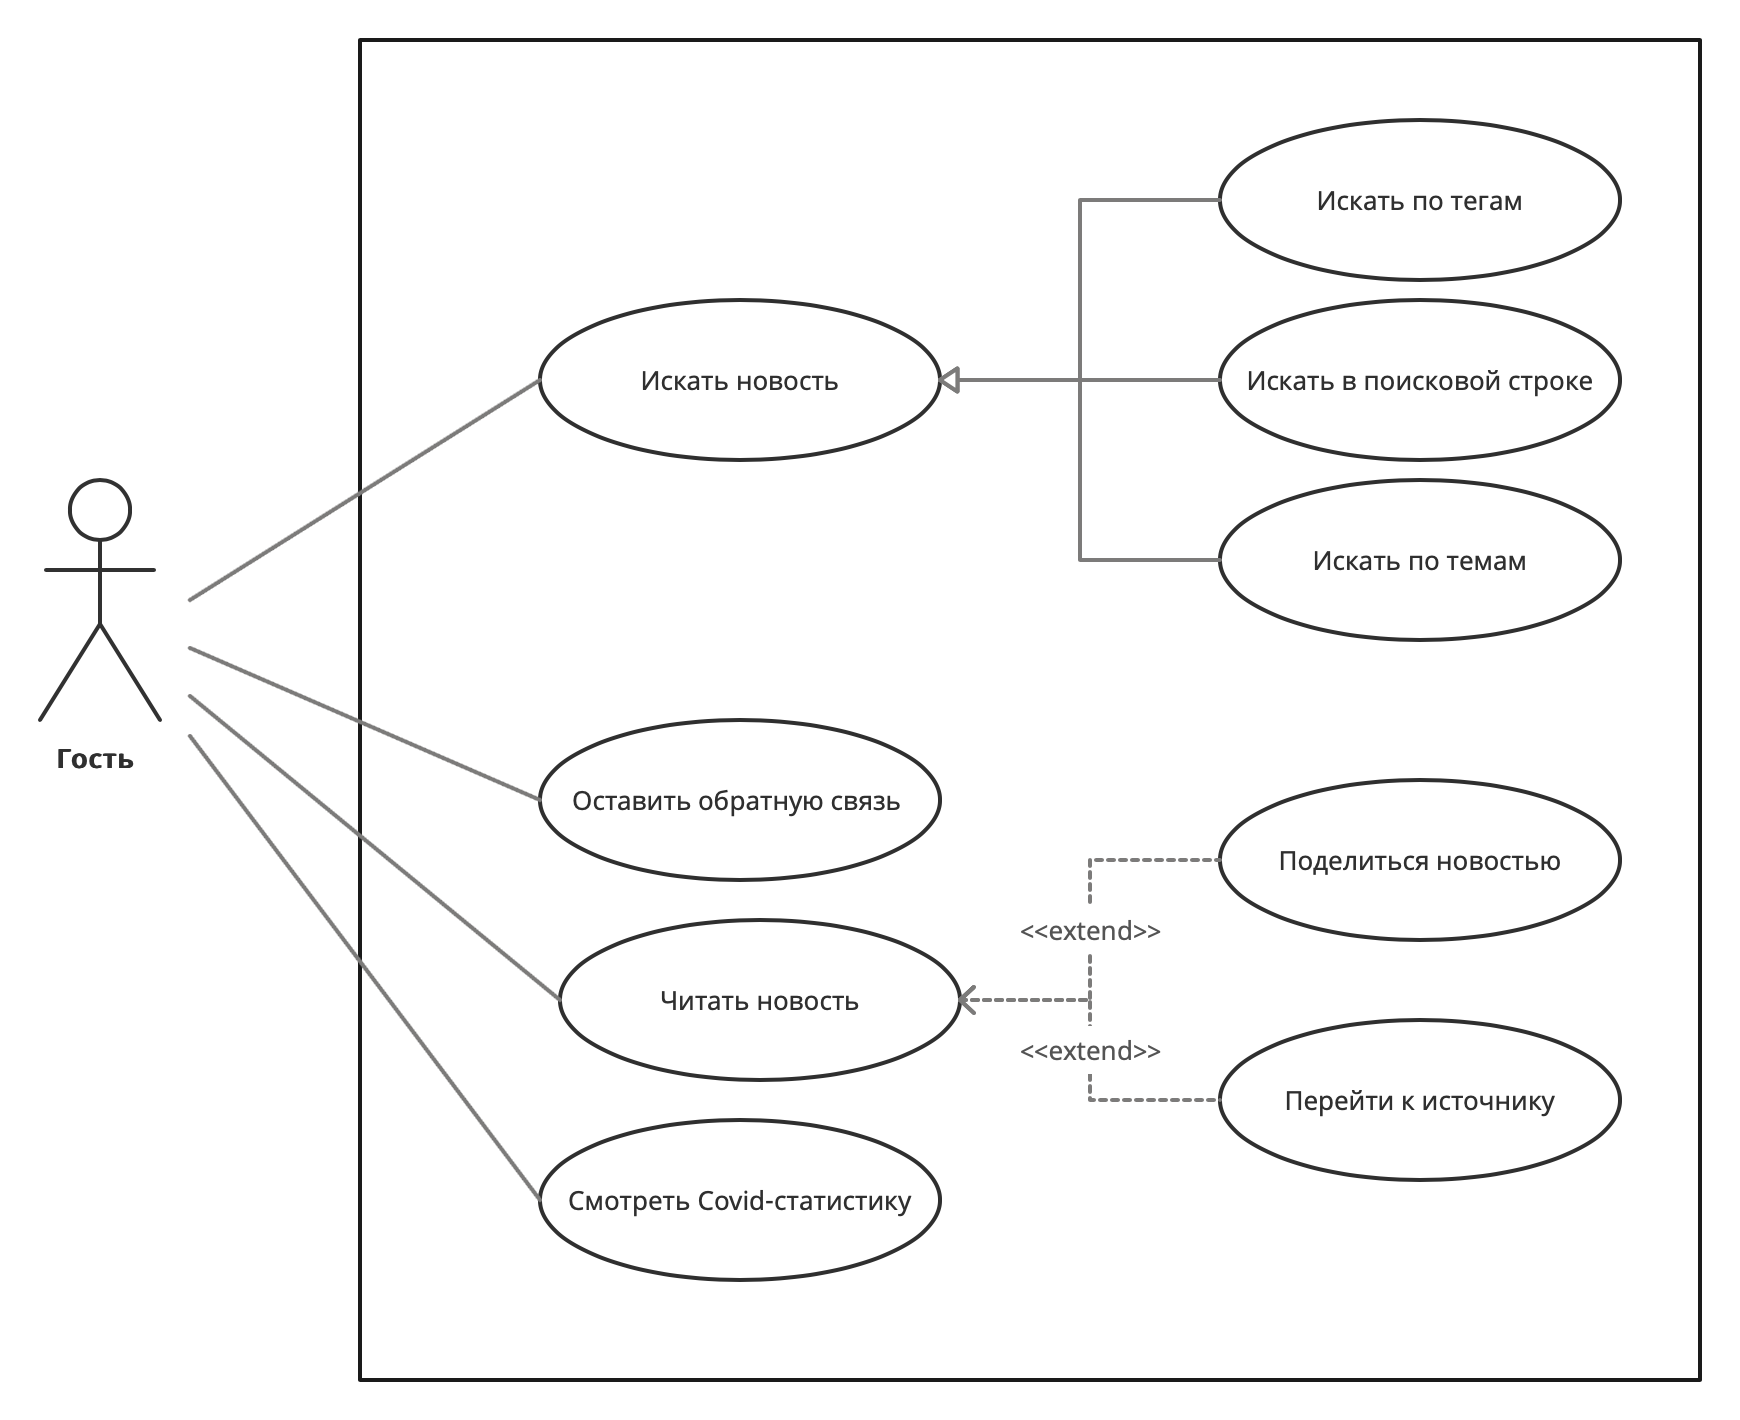
\includegraphics[scale=0.18]{img/Untitled Workspace-6}
    \end{figure}
\end{center}
\newpage
\BgThispage
\LARGE
\textbf{Risky}\\
\normalsize
\vspace{0.5cm}
\textit{Функциональные:}
\begin{enumerate}[noitemsep,topsep=0pt,parsep=0pt,partopsep=0pt]
    \item довольно стабильный процесс с низким шансом возникновения неожиданностей.
    \item используется простое и стабильное API.
    \item используется простой и предсказуемый алгоритм.
    \item используется простой и предсказуемый алгоритм.
    \item используется простой и предсказуемый алгоритм.
    \item возможен переход на несуществующую страницу из-за некорректного составления новости или истечения срока действия страницы.
    \item используется множество API, стабильность работы которых зависит от их разработчиков.
    \item возможен переход на несуществующую страницу из-за непредсказуемого поведения источника.
    \item используется чужое API, стабильность которого зависит от разработчика.
    \item предсказуемая функция с простой реализацией.
\end{enumerate}
\vspace{0.5cm}
\textit{Нефункциональные:}
\begin{enumerate}[noitemsep,topsep=0pt,parsep=0pt,partopsep=0pt]
    \item необходимо рассмотреть краевые случаи по приоритезации новостей и их корректное отображение.
    \item по умолчанию страницы легковесные, загрузка за подобное время сопровождается доп. нагрузкой на сеть или ожиданием, что может повлечь чрезмерную нагрузку на сервер в случае большого наплыва пользователей.
    \item отсутствие доп. дохода.
    \item Клименков С.В. : “Чем сильнее мы пытаемся повысить надежность системы, тем менее стабильно она работает”.
    \item передача внутреннего доступа и делегирование обязанностей сторонним лицам ( компаниям ).
    \item увеличение производительности влечет за собой доп. риски по стабильности системы.
    \item влечет увеличение использование памяти на стороне сервера и вытекающие из этого риски.
    \item простая функция, реализация которой давно изучена и используется во всех крупных проектах, имеет предсказуемый результат.
\end{enumerate}
\newpage
\BgThispage
\begin{center}
    \begin{figure}[H]
        \centering
        
\includegraphics[scale=0.2]{img/Untitled}
    \end{figure}
    \begin{figure}[H]
        \centering
        
\includegraphics[scale=0.15]{img/my_photo}
        
\includegraphics[scale=0.225]{img/dora}
    \end{figure}
\end{center}
